\documentclass{article}
\usepackage{mathtools}
\usepackage{listings}
\usepackage{qtree}
\usepackage{tikz-qtree}

\tikzset{
    black/.style={circle,draw=black,thick, minimum size=1.5em, inner sep=0},
    red/.style={circle,draw=red,thick, minimum size=1.5em, inner sep=0, fill=red!70}
}
\begin{document}
\title{CS320 Homework 3}
\author{Dustin Randall}
\maketitle

\section{Construct RBT with the following keys: 21, 19, 17, 12, 15, 9}
\subsection*{Insert 21}
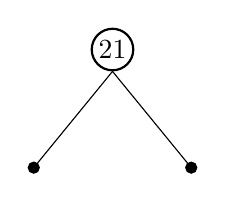
\begin{tikzpicture}[level/.style={sibling distance=20mm/#1}]
    \node [black] {21}
        child {[fill] circle (2pt)}
        child {[fill] circle (2pt)};
\end{tikzpicture} \\

\subsection*{Insert 19}
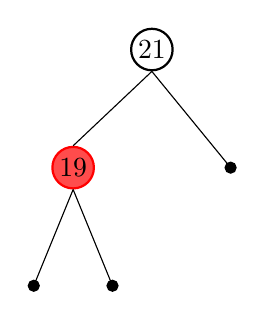
\begin{tikzpicture}[level/.style={sibling distance=20mm/#1}]
    \node[black]{21}
        child {node[red]{19}
            child {[fill] circle (2pt)}
            child {[fill] circle (2pt)}
        }
        child {[fill] circle (2pt)};
\end{tikzpicture} \\

\subsection*{Insert 17}
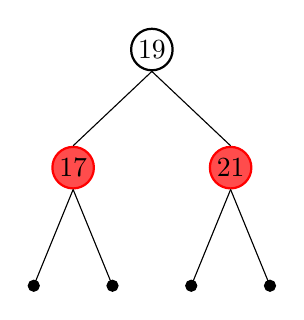
\begin{tikzpicture}[level/.style={sibling distance=20mm/#1}]
    \node[black]{19}
        child {node[red]{17}
            child {[fill] circle (2pt)}
            child {[fill] circle (2pt)}
        }
        child {node[red]{21}
            child {[fill] circle (2pt)}
            child {[fill] circle (2pt)}
        };
\end{tikzpicture} \\

\subsection*{Insert 12}
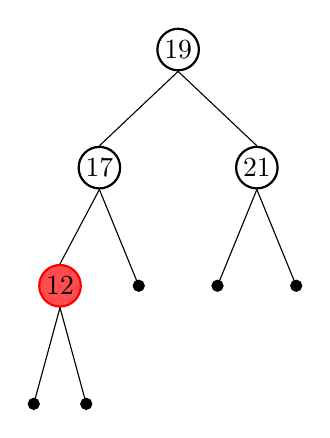
\begin{tikzpicture}[level/.style={sibling distance=20mm/#1}]
    \node[black]{19}
        child {node[black]{17}
            child {node[red]{12}
                child {[fill] circle (2pt)}
                child {[fill] circle (2pt)}
            }
            child {[fill] circle (2pt)}
        }
        child {node[black]{21}
            child {[fill] circle (2pt)}
            child {[fill] circle (2pt)}
        };
\end{tikzpicture} \\

\subsection*{Insert 15}
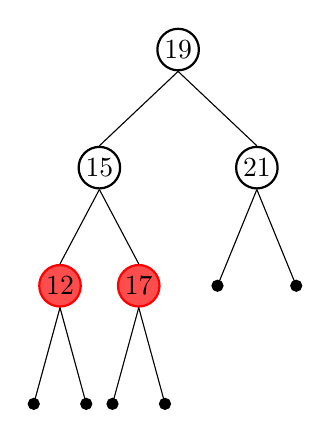
\begin{tikzpicture}[level/.style={sibling distance=20mm/#1}]
    \node[black]{19}
        child {node[black]{15}
            child {node[red]{12}
                child {[fill] circle (2pt)}
                child {[fill] circle (2pt)}
            }
            child {node[red] {17}
                child {[fill] circle (2pt)}
                child {[fill] circle (2pt)}
            }
        }
        child {node[black]{21}
            child {[fill] circle (2pt)}
            child {[fill] circle (2pt)}
        };
\end{tikzpicture} \\

\subsection*{Insert 9}

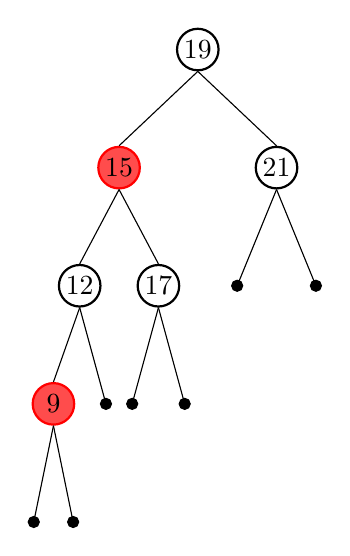
\begin{tikzpicture}[level/.style={sibling distance=20mm/#1}]
    \node[black]{19}
        child {node[red]{15}
            child {node[black]{12}
                child {node[red] {9}
                    child {[fill] circle (2pt)}
                    child {[fill] circle (2pt)}
                }
                child {[fill] circle (2pt)}
            }
            child {node[black] {17}
                child {[fill] circle (2pt)}
                child {[fill] circle (2pt)}
            }
        }
        child {node[black]{21}
            child {[fill] circle (2pt)}
            child {[fill] circle (2pt)}
        };
\end{tikzpicture} \\

\section{Delete the nodes of the RBT in the following order: 2, 5, 1, 14, 11, 15, 7, 8}
\subsection*{Initial Tree}
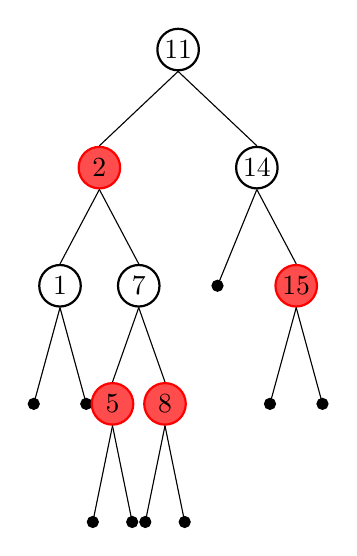
\begin{tikzpicture}[level/.style={sibling distance=20mm/#1}]
    \node[black]{11}
        child {node[red]{2}
            child {node[black]{1}
                child {[fill] circle (2pt)}
                child {[fill] circle (2pt)}
            }
            child {node[black]{7}
                child {node[red] {5}
                    child {[fill] circle (2pt)}
                    child {[fill] circle (2pt)}
                }
                child {node[red]{8}
                    child {[fill] circle (2pt)}
                    child {[fill] circle (2pt)}
                }
            }
        }
        child {node[black]{14}
            child {[fill] circle (2pt)}
            child {node[red]{15}
                child {[fill] circle (2pt)}
                child {[fill] circle (2pt)}
            }
        };
\end{tikzpicture} \\

\subsection*{Delete 2}
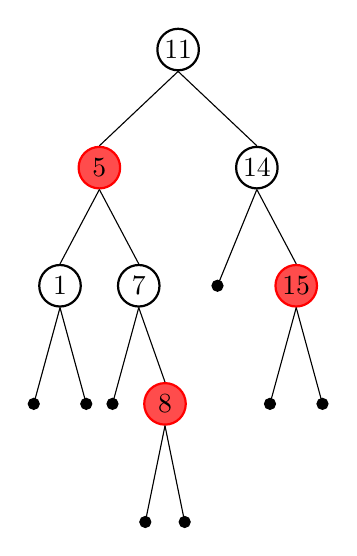
\begin{tikzpicture}[level/.style={sibling distance=20mm/#1}]
    \node[black]{11}
        child {node[red]{5}
            child {node[black]{1}
                child {[fill] circle (2pt)}
                child {[fill] circle (2pt)}
            }
            child {node[black]{7}
                child {[fill] circle (2pt)}
                child {node[red]{8}
                    child {[fill] circle (2pt)}
                    child {[fill] circle (2pt)}
                }
            }
        }
        child {node[black]{14}
            child {[fill] circle (2pt)}
            child {node[red]{15}
                child {[fill] circle (2pt)}
                child {[fill] circle (2pt)}
            }
        };
\end{tikzpicture} \\

\subsection*{Delete 5}
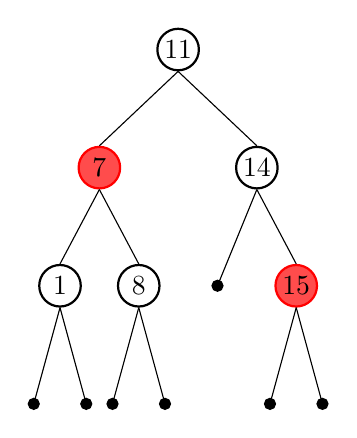
\begin{tikzpicture}[level/.style={sibling distance=20mm/#1}]
    \node[black]{11}
        child {node[red]{7}
            child {node[black]{1}
                child {[fill] circle (2pt)}
                child {[fill] circle (2pt)}
            }
            child {node[black]{8}
                child {[fill] circle (2pt)}
                child {[fill] circle (2pt)}
            }
        }
        child {node[black]{14}
            child {[fill] circle (2pt)}
            child {node[red]{15}
                child {[fill] circle (2pt)}
                child {[fill] circle (2pt)}
            }
        };
\end{tikzpicture} \\

\subsection*{Delete 1}
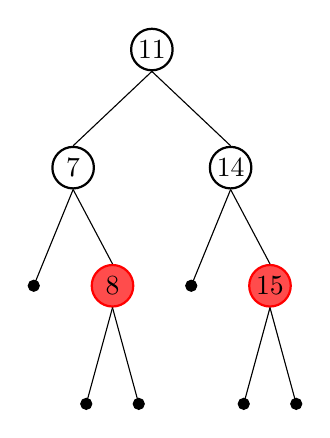
\begin{tikzpicture}[level/.style={sibling distance=20mm/#1}]
    \node[black]{11}
        child {node[black]{7}
            child {[fill] circle (2pt)}
            child {node[red]{8}
                child {[fill] circle (2pt)}
                child {[fill] circle (2pt)}
            }
        }
        child {node[black]{14}
            child {[fill] circle (2pt)}
            child {node[red]{15}
                child {[fill] circle (2pt)}
                child {[fill] circle (2pt)}
            }
        };
\end{tikzpicture} \\

\subsection*{Delete 14}
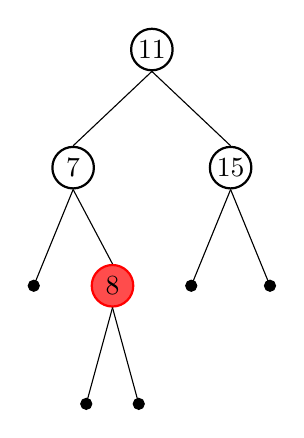
\begin{tikzpicture}[level/.style={sibling distance=20mm/#1}]
    \node[black]{11}
        child {node[black]{7}
            child {[fill] circle (2pt)}
            child {node[red]{8}
                child {[fill] circle (2pt)}
                child {[fill] circle (2pt)}
            }
        }
        child {node[black]{15}
            child {[fill] circle (2pt)}
            child {[fill] circle (2pt)}
        };
\end{tikzpicture} \\

\subsection*{Delete 11}
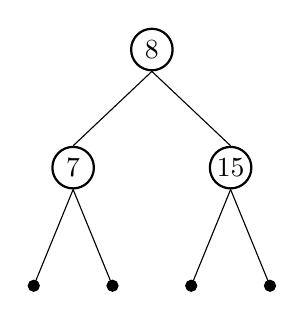
\begin{tikzpicture}[level/.style={sibling distance=20mm/#1}]
    \node[black]{8}
        child {node[black]{7}
            child {[fill] circle (2pt)}
            child {[fill] circle (2pt)}
        }
        child {node[black]{15}
            child {[fill] circle (2pt)}
            child {[fill] circle (2pt)}
        };
\end{tikzpicture} \\

\subsection*{Delete 15}
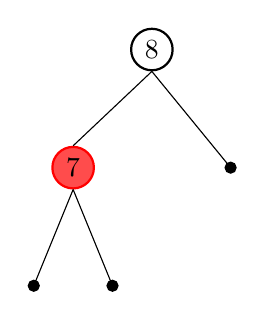
\begin{tikzpicture}[level/.style={sibling distance=20mm/#1}]
    \node[black]{8}
        child {node[red]{7}
            child {[fill] circle (2pt)}
            child {[fill] circle (2pt)}
        }
        child {[fill] circle (2pt)};
\end{tikzpicture} \\

\subsection*{Delete 7}
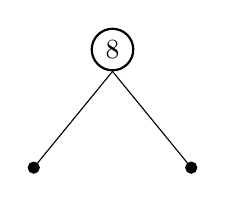
\begin{tikzpicture}[level/.style={sibling distance=20mm/#1}]
    \node[black]{8}
        child {[fill] circle (2pt)}
        child {[fill] circle (2pt)};
\end{tikzpicture} \\

\subsection*{Delete 8}

\section{Trace the one-pass construction of a B-Tree with t=2 with the following nodes: S, G, W, H, O, U, M, A, C, X, P}

\subsection*{Insert S}
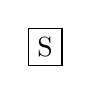
\begin{tikzpicture}[level/.style={sibling distance=25mm/#1}]
    \node[rectangle, draw]{S};
\end{tikzpicture}

\subsection*{Insert G}

\begin{tikzpicture}[level/.style={sibling distance=25mm/#1}]
    \node[rectangle, draw]{G S};
\end{tikzpicture}

\subsection*{Insert W}

\begin{tikzpicture}[level/.style={sibling distance=25mm/#1}]
    \node[rectangle, draw]{G S W};
\end{tikzpicture}

\subsection*{Insert H}
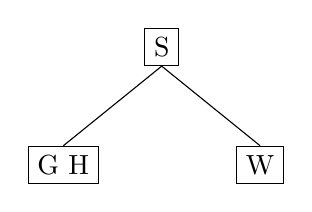
\begin{tikzpicture}[level/.style={sibling distance=25mm/#1}]
    \node[rectangle, draw]{S}
        child {node[rectangle, draw]{G H}}
        child {node[rectangle, draw]{W}};
\end{tikzpicture}

\subsection*{Insert O}
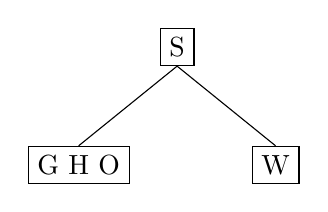
\begin{tikzpicture}[level/.style={sibling distance=25mm/#1}]
    \node[rectangle, draw]{S}
        child {node[rectangle, draw]{G H O}}
        child {node[rectangle, draw]{W}};
\end{tikzpicture}

\subsection*{Insert U}
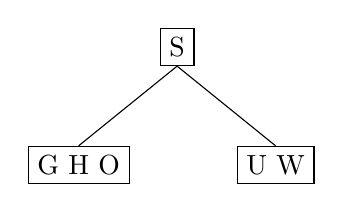
\begin{tikzpicture}[level/.style={sibling distance=25mm/#1}]
    \node[rectangle, draw]{S}
        child {node[rectangle, draw]{G H O}}
        child {node[rectangle, draw]{U W}};
\end{tikzpicture}

\subsection*{Insert M}
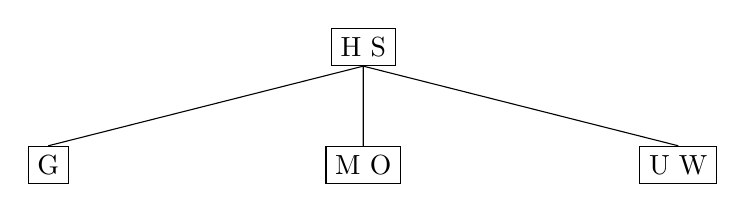
\begin{tikzpicture}[level/.style={sibling distance=40mm/#1}]
    \node[rectangle, draw]{H S}
        child {node[rectangle, draw]{G}}
        child {node[rectangle, draw]{M O}}
        child {node[rectangle, draw]{U W}};
\end{tikzpicture}

\subsection*{Insert A}
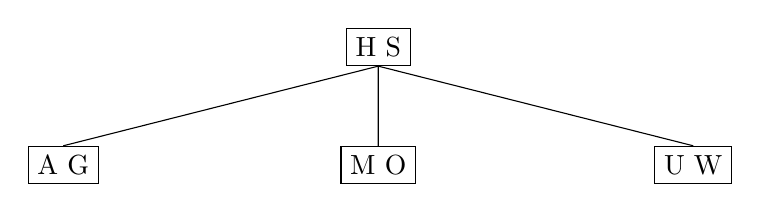
\begin{tikzpicture}[level/.style={sibling distance=40mm/#1}]
    \node[rectangle, draw]{H S}
        child {node[rectangle, draw]{A G}}
        child {node[rectangle, draw]{M O}}
        child {node[rectangle, draw]{U W}};
\end{tikzpicture}

\subsection*{Insert C}
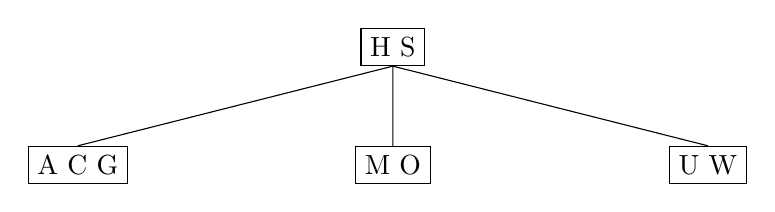
\begin{tikzpicture}[level/.style={sibling distance=40mm/#1}]
    \node[rectangle, draw]{H S}
        child {node[rectangle, draw]{A C G}}
        child {node[rectangle, draw]{M O}}
        child {node[rectangle, draw]{U W}};
\end{tikzpicture}

\subsection*{Insert X}
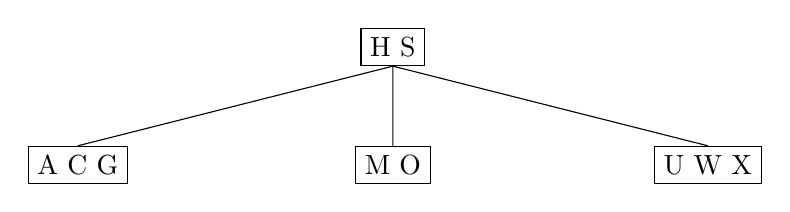
\begin{tikzpicture}[level/.style={sibling distance=40mm/#1}]
    \node[rectangle, draw]{H S}
        child {node[rectangle, draw]{A C G}}
        child {node[rectangle, draw]{M O}}
        child {node[rectangle, draw]{U W X}};
\end{tikzpicture}

\subsection*{Insert P}
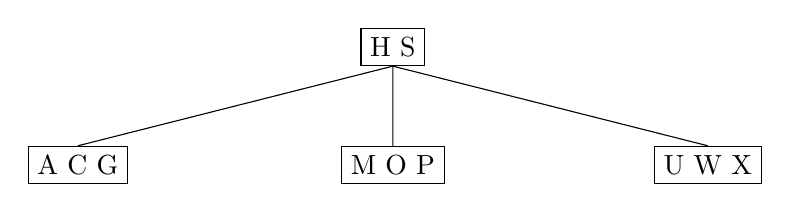
\begin{tikzpicture}[level/.style={sibling distance=40mm/#1}]
    \node[rectangle, draw]{H S}
        child {node[rectangle, draw]{A C G}}
        child {node[rectangle, draw]{M O P}}
        child {node[rectangle, draw]{U W X}};
\end{tikzpicture}

\section{Delete the following nodes in order from the initial B-Tree: T, G, F, O}
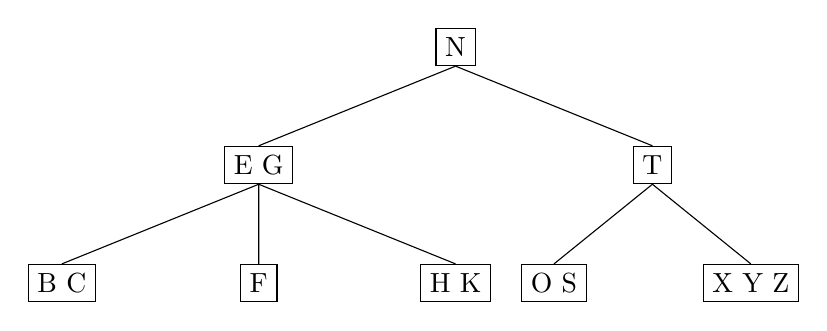
\begin{tikzpicture}[level/.style={sibling distance=50mm/#1}]
    \node[rectangle, draw]{N}
        child {node[rectangle, draw]{E G}
            child {node[rectangle, draw]{B C}}
            child {node[rectangle, draw]{F}}
            child {node[rectangle, draw]{H K}}
        }
        child {node[rectangle, draw]{T}
            child {node[rectangle, draw]{O S}}
            child {node[rectangle, draw]{X Y Z}}
        };
\end{tikzpicture}

\subsection*{Delete T}
\subsubsection*{Borrow G from Left Child}
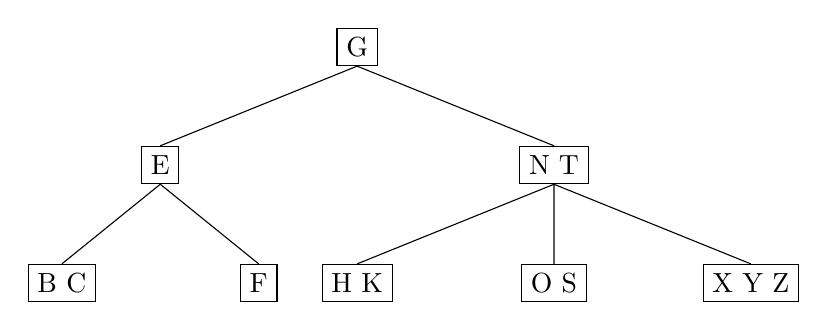
\begin{tikzpicture}[level/.style={sibling distance=50mm/#1}]
    \node[rectangle, draw]{G}
        child {node[rectangle, draw]{E}
            child {node[rectangle, draw]{B C}}
            child {node[rectangle, draw]{F}}
        }
        child {node[rectangle, draw]{N T}
            child {node[rectangle, draw]{H K}}
            child {node[rectangle, draw]{O S}}
            child {node[rectangle, draw]{X Y Z}}
        };
\end{tikzpicture}

\subsubsection*{Swap Predecessor S with T}
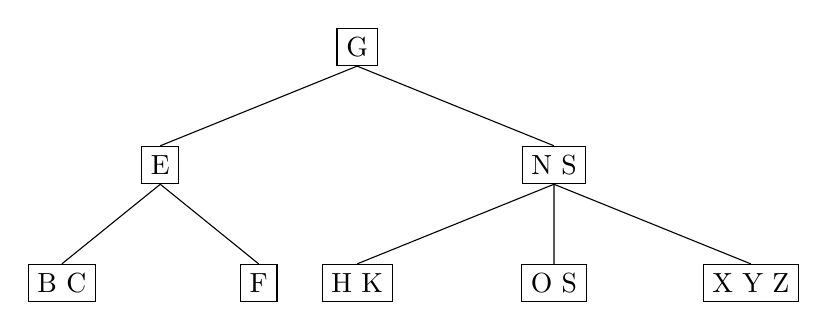
\begin{tikzpicture}[level/.style={sibling distance=50mm/#1}]
    \node[rectangle, draw]{G}
        child {node[rectangle, draw]{E}
            child {node[rectangle, draw]{B C}}
            child {node[rectangle, draw]{F}}
        }
        child {node[rectangle, draw]{N S}
            child {node[rectangle, draw]{H K}}
            child {node[rectangle, draw]{O S}}
            child {node[rectangle, draw]{X Y Z}}
        };
\end{tikzpicture}

\subsubsection*{Delete S from Leaf}
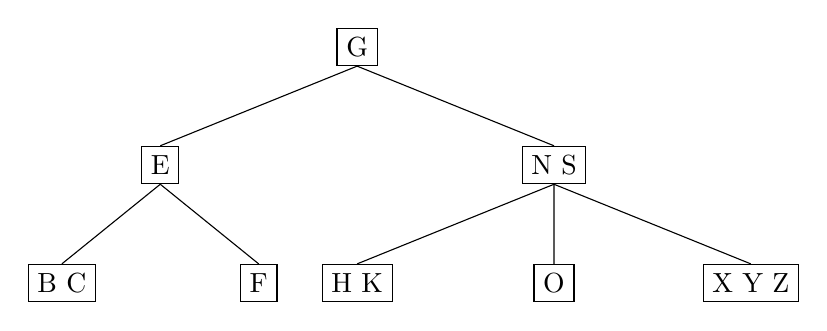
\begin{tikzpicture}[level/.style={sibling distance=50mm/#1}]
    \node[rectangle, draw]{G}
        child {node[rectangle, draw]{E}
            child {node[rectangle, draw]{B C}}
            child {node[rectangle, draw]{F}}
        }
        child {node[rectangle, draw]{N S}
            child {node[rectangle, draw]{H K}}
            child {node[rectangle, draw]{O}}
            child {node[rectangle, draw]{X Y Z}}
        };
\end{tikzpicture}

\subsection*{Delete G}
\subsubsection*{Swap G with Successor H}
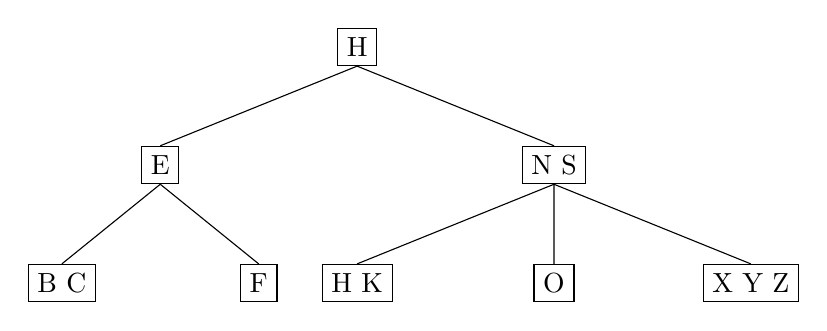
\begin{tikzpicture}[level/.style={sibling distance=50mm/#1}]
    \node[rectangle, draw]{H}
        child {node[rectangle, draw]{E}
            child {node[rectangle, draw]{B C}}
            child {node[rectangle, draw]{F}}
        }
        child {node[rectangle, draw]{N S}
            child {node[rectangle, draw]{H K}}
            child {node[rectangle, draw]{O}}
            child {node[rectangle, draw]{X Y Z}}
        };
\end{tikzpicture}

\subsubsection*{Delete H from Leaf}
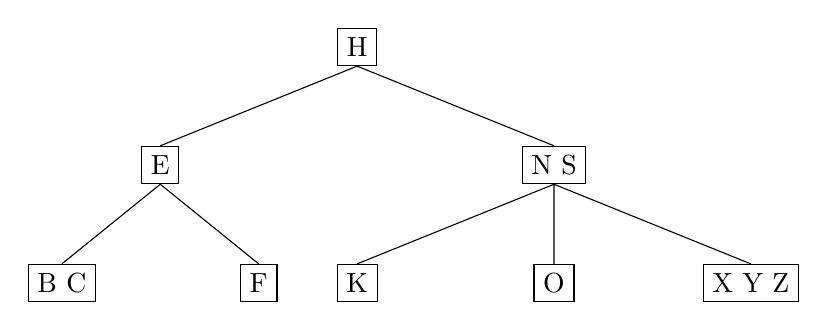
\begin{tikzpicture}[level/.style={sibling distance=50mm/#1}]
    \node[rectangle, draw]{H}
        child {node[rectangle, draw]{E}
            child {node[rectangle, draw]{B C}}
            child {node[rectangle, draw]{F}}
        }
        child {node[rectangle, draw]{N S}
            child {node[rectangle, draw]{K}}
            child {node[rectangle, draw]{O}}
            child {node[rectangle, draw]{X Y Z}}
        };
\end{tikzpicture}

\subsection*{Delete F}
\subsubsection{Borrow N from Right Sibling}
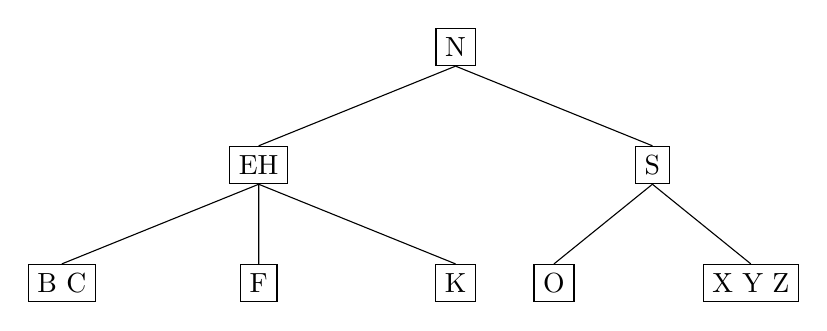
\begin{tikzpicture}[level/.style={sibling distance=50mm/#1}]
    \node[rectangle, draw]{N}
        child {node[rectangle, draw]{EH}
            child {node[rectangle, draw]{B C}}
            child {node[rectangle, draw]{F}}
            child {node[rectangle, draw]{K}}
        }
        child {node[rectangle, draw]{S}
            child {node[rectangle, draw]{O}}
            child {node[rectangle, draw]{X Y Z}}
        };
\end{tikzpicture}

\subsubsection{Borrow C from Left Sibling}
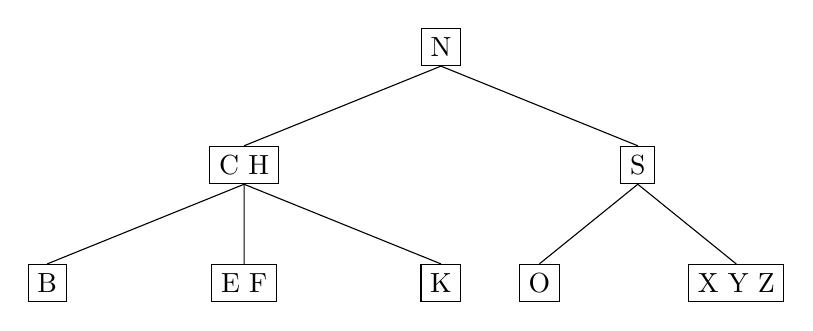
\begin{tikzpicture}[level/.style={sibling distance=50mm/#1}]
    \node[rectangle, draw]{N}
        child {node[rectangle, draw]{C H}
            child {node[rectangle, draw]{B}}
            child {node[rectangle, draw]{E F}}
            child {node[rectangle, draw]{K}}
        }
        child {node[rectangle, draw]{S}
            child {node[rectangle, draw]{O}}
            child {node[rectangle, draw]{X Y Z}}
        };
\end{tikzpicture}

\subsubsection{Remove F from Leaf}
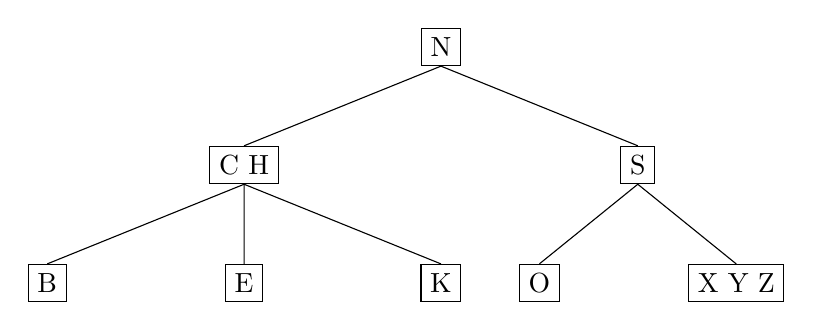
\begin{tikzpicture}[level/.style={sibling distance=50mm/#1}]
    \node[rectangle, draw]{N}
        child {node[rectangle, draw]{C H}
            child {node[rectangle, draw]{B}}
            child {node[rectangle, draw]{E}}
            child {node[rectangle, draw]{K}}
        }
        child {node[rectangle, draw]{S}
            child {node[rectangle, draw]{O}}
            child {node[rectangle, draw]{X Y Z}}
        };
\end{tikzpicture}

\subsection{Delete O}
\subsubsection{Borrow H from Left Sibling}
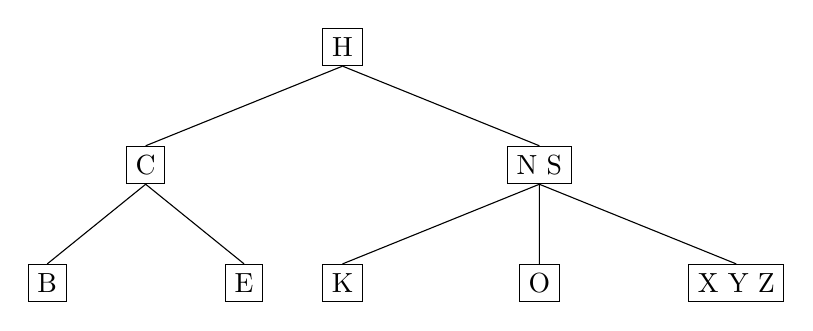
\begin{tikzpicture}[level/.style={sibling distance=50mm/#1}]
    \node[rectangle, draw]{H}
        child {node[rectangle, draw]{C}
            child {node[rectangle, draw]{B}}
            child {node[rectangle, draw]{E}}
        }
        child {node[rectangle, draw]{N S}
            child {node[rectangle, draw]{K}}
            child {node[rectangle, draw]{O}}
            child {node[rectangle, draw]{X Y Z}}
        };
\end{tikzpicture}

\subsubsection{Borrow X from Right Sibling}
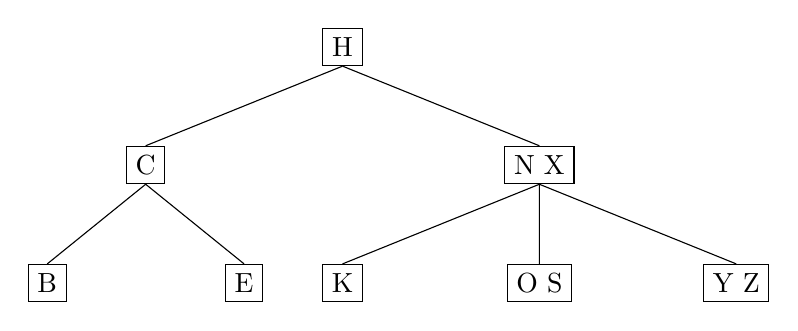
\begin{tikzpicture}[level/.style={sibling distance=50mm/#1}]
    \node[rectangle, draw]{H}
        child {node[rectangle, draw]{C}
            child {node[rectangle, draw]{B}}
            child {node[rectangle, draw]{E}}
        }
        child {node[rectangle, draw]{N X}
            child {node[rectangle, draw]{K}}
            child {node[rectangle, draw]{O S}}
            child {node[rectangle, draw]{Y Z}}
        };
\end{tikzpicture}

\subsubsection{Delete O From Leaf}
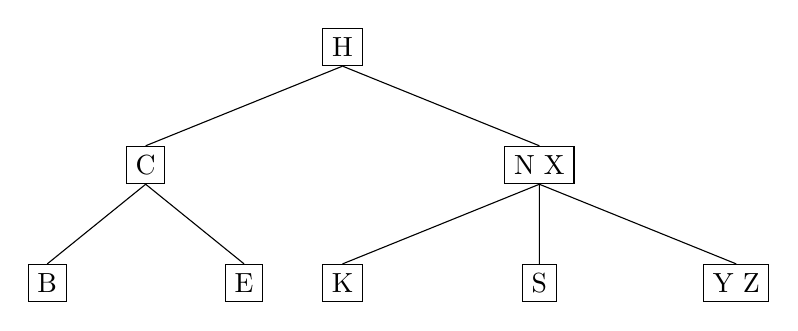
\begin{tikzpicture}[level/.style={sibling distance=50mm/#1}]
    \node[rectangle, draw]{H}
        child {node[rectangle, draw]{C}
            child {node[rectangle, draw]{B}}
            child {node[rectangle, draw]{E}}
        }
        child {node[rectangle, draw]{N X}
            child {node[rectangle, draw]{K}}
            child {node[rectangle, draw]{S}}
            child {node[rectangle, draw]{Y Z}}
        };
\end{tikzpicture}


\section{Explain BTreeMin and BTreeSuccessor}
\subsection*{BTreeMin}
Given a node, traverse down the left-most child until there are no more children.
Once there, return the index of the smallest element in that node, along with a pointer to the node.
\subsection*{BTreeSuccessor}
If I has a right child, the successor is the BTreeMin of the right child.
Otherwise, while we're the right most child of our parent, get the next parent.
Finally after finding a non-right-most parent, return the key after our node.
If we run out of parents, return null.

\subsection*{Pseudocode}
\begin{lstlisting}
(Node, Index) BTreeMin(root) {
    while(root.Children.Count > 0) {
        root = root.Children[0]; // DISK_READ
    }
    // assuming keys are in order
    return (root, 0);
    // alternatively, return (root, min(root.Keys))
}

(successor_node, j) BTreeSuccessor(node, i) {
    if(node.Children.Count > i) {
        return BTreeMin(node.Children[i + 1]);
    }
    //in a leaf node, and successor is in this node
    if(node.IsLeaf && i + 1 < node.Keys.Count) {
        return (node, i + 1);
    } else {
        Node parent = node.Parent; // DISK_READ
        pIndex = parent.FindIndex(node);
        while(pIndex == parent.Keys.Count) {
            node = parent;
            parent = node.Parent; // DISK_READ
            if(parent == null) return null;
            pIndex = parent.FindIndex(node);
        }
        return (parent, pIndex);
    }
}
\end{lstlisting}
\end{document}